\chapter{Method}

We took a systems design and implementation approach in the development of our system, designing and implementing a working prototype system. Our plan of attack was formulated in accordance with the ultimate goal -- a working prototype system after 3 months of work. 

\section{Phases and design decisions}

The main project phases were
%
\begin{enumerate}

% Design phase
\item Phase: Design
\begin{enumerate}
\item Overall system design. Outline the concept and interaction of components.
\item Design and implementation of cryptographic protocols for authentication, re-keying and data transfer.
\item System component design
\begin{enumerate}
\item Design sensor prototype software.
\item Design sink and authentication server software.
\end{enumerate}
\end{enumerate}

% Crypto implementaiton phase
\item Phase: Implementation of cryptographic primitives
\begin{enumerate}
\item AES block cipher encryption and decryption
\item CBC-mode encryption and decryption
\item CMAC
\end{enumerate}

% System implementaiton phase
\item Phase: Implementation and integration
\begin{enumerate}
\item Authentication, re-keying and transfer protocol implementation
\item tsensor development
\item sink and authentication server development
\item System integration
\end{enumerate}

% Integration and testing
\item Phase: Unit and system tests in a test bed system

\end{enumerate}
%
Phases 2 and 3 overlapped in part.


\subsection{System design decisions}

The main requirements for the TSense system were
%
\begin{enumerate}
\item The system should be as simple as possible, while at the same time giving reasonable security guarantees (confidentiality and integrity).
\item The cryptographic primitives should be as strong as possible, within the limits posed by the resource constrained sensor hardware.
\item All cryptographic algorithms should be open and non-proprietary.
\item System integrity should be ensured. In particular, an adversary should not be able to insert cloned sensors or simulate multiple sensors. 
\item The sensor should be compact and cheap as possible, almost a disposable unit. 
\end{enumerate}

\subsubsection{Simplicity}

Client/server systems are the simplest networked systems to design and implement. We decided upon this configuration for our test system. The client is a sensor/client pair, while the server is the sink. We decided to use a separate authentication server to allow for system scalability by deploying multiple sink servers; a single authentication server maintains the requirement that the secret device keys are distributed amongst the fewest nodes possible.

\subsubsection{Security}

We initially considered public key crypto algorithms, which would have allowed us to simplify the system further by excluding the authentication server. In such a system, each tsensor would hold a public/private keypair and the public key could be safely distributed amongst all sinks. Factoring and discrete logarithm based public key algorithms require very large keys -- 1024 bits at least -- rendering this approach impractical on the ATmega328. However, elliptic curve algorithms \cite{menezes1995,ieee-1363-2000}, such as ECEG \cite{}, ECDH \cite{} and ECDSA \cite{johnson2001a}, require much shorter keys, even as short as XXXX bits \cite{} \textbf{SEE ALSO \cite{NIST-recommended-elliptic-curves-1999}}, meaning that such algorithms may be practical on small resource constrained devices.  \textbf{CITE JOHNSON, HANKERSON.}
%
In the end, we decided to use only symmetric (private key) algorithms, mainly for the reasons of expediency. Only single cryptographic primitive is required in our approach, which saves on coding and testing effort as compared to implementing an additional set of public key algorithms.

Security objectives are often stated in terms of the CIA trilogy -- \textit{confidentiality}, \textit{integrity} and \textit{availability}. 
%
Integrity is our primary concern. That is, no intermediary node, including the client holding the tsensor, should be able to modify messages (within computational bounds) undetected. Confidentiality is a secondary goal, but easily achieved by standard symmetric cryptographic primitives at tsensor and sink. Using such primitives, we can say that no active or passive adversary should be able (within computational bounds) to extract the transmitted information on the route between tsensor and sink.
%
We do not address availability issues -- denial-of-service, routing attacks and the like -- in our work.

\subsubsection{Open cryptographic algorithms}

Shannon's maxim "the enemy knows the system" is often a prudent assumption. Kerckhoffs' law\footnote{\textit{La cryptographie militaire}, Journal des sciences militaires, vol. IX, pp. 5--38, 161–191, 1883} states roughly the same principles, demonstrating the longevity of open design. Briefly, these assumptions dictate design principles where we assume any adversary, internal or external, knows intimately all aspects of the system, except for cryptographic keys. In particular, this includes knowledge of the algorithms and protocols employed. Layered security is certainly prudent in most practical scenarios, whereas reliance on security by obscurity is usually regarded as poor practice. We assume open cryptographic protocols in our design, basing the security solely on secret keys. For this reason, we selected the Rijndael block cipher, which was selected as the Advanced Encryption Standard (AES) in an open competition \cite{}.

\subsubsection{System integrity}

The Sybil attack \cite{Douceur2002} is a very real threat to any distributed system. In this attack, an adversary simulates multiple colluding nodes on a single (or relatively few) highly capable platform. An adversary could easily simulate even thousands of tsensors on a high-end PC, unless measures were taken to prevent such an attack. Cloning and multiple insertion of a single sensor is a related, but less damaging, attack.
%
Various solutions have been proposed for the Sybil attack, but the only absolute one is using strong and unforgeable node identities. This is the approach we take. Each tsensor has a strong and unforgeable (within computational bounds) identity in the form of a globally unique public ID and a 128-bit secret key (randomly generated), shared only with the authentication service. The identification and authentication protocol, described in Section~\ref{}, ensures (within computational bounds) that no more than one instance of each tsensor can be active in the system at any given time. Since the trusted authentication server holds the private keys and identities of all sensors manufactured, we can claim that no adversary can simulate a non-existent sensor.

System integrity requirements also dictate that the secret sensor keys should exist on as few nodes as possible. Each key is unique and permanently "burned" onto the tsensor device. The symmetric nature of the authentication protocol requires the key to be present on at least one other node. Minimal distribution of the secret key is achieved by using a trusted third party, the authentication server tauth, as described in Section~\ref{}.

\subsubsection{Small and inexpensive sensor}

We selected an embedded microcontroller, the Atmel ATmega328, widely used in sensor nodes \cite{} amongst other applications. Our development platform is an Arduino Duemilanove experimentation board with an ATmega328 in a 28-pin DIL package. The board is about 5x7 cm in size.
The cost of this board is \$29.95 (+ shipping and import costs) in quantities of one from \url{http://www.sparkfun.com} in june 2010. 
%
Production sensors would use a much smaller custom PCB and a surface mount version of the processor. ATmega328 (in the 28-pin package) cost \$4.40 in quantities of 100+ from \url{http://www.sparkfun.com} in june 2010. Bulk manufacture of an ATmega328-based tsensor device is estimated as starting at about \$10, depending on the type and sophistication of the embedded sensors. Estimated size for a production unit is less than 2x2 cm, using a surface mount ATmega328 package. Even smaller sizes can be achieved using custom ICs. 

\section{The TSense system}

\begin{figure}
\begin{center}
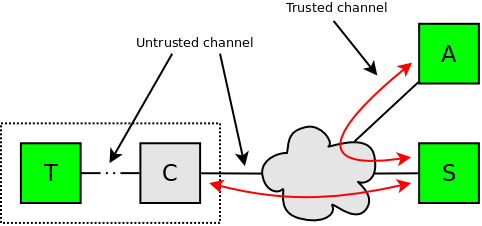
\includegraphics[width=0.6\textwidth]{figures/sys-overview.png} 
\end{center}
\caption{System overview. Interaction of the entities of the TSensor system. Green: Trusted entities. Gray: Untrusted entities (compromizable), Black channels: Untrusted, Red channels: Secure.}
\label{fig:sys-overview}
\end{figure}

The TSense system is shown in its simplest form in Figure~\ref{fig:sys-overview}. The module types are
%
\begin{description}

\item \textbf{T}: The trusted sensor -- \textit{tsensor} -- measures some array of quantities, e.g.\ temperature, pollutant particle count or luminosity, and publishes in an authenticated manner to a client ($C$). The published results may additionally be encrypted. tsensor would be a tamper-proof unit in a production setting.

\item \textbf{C}: The client -- \textit{tsclient} -- hosts the sensor, e.g.\ physically attached or USB-connected. The client is the corruptible (adversary controlled) entity in our model, as further discussed in Section~\ref{sec:sec-goals}. A honest client will always forward measurements unmodified to the sink $S$, whereas a corrupted $C$ may attempt modify the readings.

\item \textbf{S}: The sink server -- \textit{tsink} -- collects measurements forwarded from a number of client nodes over TCP/IP. A network may include multiple networked sinks to achieve some degree of scalability. In such a system, each of the sinks is a \textit{clusterhead} for a number of clients. In this work, we regard all $S$ to be trusted. %This is a simplifying assumption that will be relaxed in future work.

\item \textbf{A}: The authentication server -- \textit{tauth} -- is the trusted third party (see Section~\ref{}) in our system and handles authentication of sensor/client pairs at time of insertion into a working measurement network. 
%Even though we regard the $S$ to be trusted, it is a prudent measure to limit the distribution of sensor private keys. In our model, we limit the distribution of the private sensor keys to $T$ and $A$ nodes. 
We regard tauth to be incorruptible (unconditionally). A single tauth is assumed in the TSense system, which is a reasonable assumption from a scalability standpoint, since authentication takes place much less frequently than data collection.

\end{description}

Communications channels are as follows:
%
\begin{description}
\item {$tsensor \longleftrightarrow tsclient$:}
The tsensor and tsclient communicate over a serial link, provided by an USB-serial emulator. The tsclient, and by extension both of its communications channels, are considered untrusted. The tsensor and tsclient communicate using a dedicated communications protocol (partly secured by the tsensor), further described in Section~\ref{}. However, tsclient plays no part in the system security.

\item {$tsclient \longleftrightarrow tsink$:}
The tsclient and tsink communicate over an IP network, using TCP/IP and a set of dedicated protocols described in Section~\ref{}. Other transport layer protocols than TCP may be used; our decision to use standard socket communications was merely one of convenience. In particular, we may consider unreliable wireless communications protocols in our future work. tsclient and tsink use a standard unencrypted TCP connection; all security is provided by tsensor/sink operations, rendering critical operations inaccessible and unmodifiable (within computational bounds) by the untrusted tsclient and any third parties.

\item {$tsink \longleftrightarrow tauth$:}
The tsink and tauth communicate over an IP network, using Transport Layer Security (TLS) \cite{} and TCP-IP. TLS provides strong mutual authentication, confidentiality and integrity for message transfer between these two critical system types. Both have installed X.509 certificates and hold each others public keys.
%A bit of security-by-obscurity can be assumed by using non-standard ports.  

\end{description}

\section{Cryptographic primitives}

\subsection{The block cipher -- AES}

A symmetric block or stream cipher is the workhorse of any confidentiality-preserving transfer protocol. 
%
Stream ciphers are generally faster than block ciphers, but harder to handle correctly. In particular, care must be taken to never re-use initialization vectors (IVs) when using stream ciphers. Examples of stream ciphers are e.g.\ found in the \textit{eCRYPT} stream cipher portfolio\footnote{\url{http://www.ecrypt.eu.org/stream}}. 
%
Block ciphers include the industry-standard AES (Rijndael) \shortcite{fips-197-2001,daemen1999,daemen2000,gladman2001}, Blowfish \shortcite{schneier1997}, Skipjack \shortcite{skipjack-1998,brickell1993} and TEA/XTEA \shortcite{wheeler1995,needham1997}\footnote{See  \url{http://www.users.zetnet.co.uk/hopwood/crypto/scan/cs.html} for a comprehensive list of block and stream ciphers}.

We selected the Rijndael algorithm (AES standard) \shortcite{fips-197-2001}, with a 128-bit key length, for our prototype. This is the weakest AES variant, but the key length preserves valuable space on the tsensor device. It is however quite strong enough for our purposes, since no known attacks exist against AES, except for reduced round (reduced strength) variants \cite{}. One of the design requirements of the Rijndael algorithm was that it should be implementable on small 8-bit devices with limited memory. The algorithm has been implemented successfully on small devices, such as the YubiKey\footnote{\url{http://www.yubico.com/products/yubikey}} one time password generator.

We decided to write our own implementation of AES, rather than use an existing library. This choice was made in order to be able to support the various platforms in our system with the same code base. Our implementation of AES is close to the byte-oriented pseudocode published in the AES standard \shortcite{fips-197-2001}, although tuned for performance. More efficient implementations of AES are feasible using word oriented algorithms, in essence pre-computing the AES round functions in four lookup tables and reducing the encryption and decryption processes to four table lookups and XORs \cite[Section 5.2]{daemen1999}. However, such implementations depend on rather large lookup tables, a drawback for memory constrained devices. Further, such algorithms are highly architecture dependent and therefore tricky to write in a multi-platform manner. We therefore decided to restrict our implementation to one close to the byte-oriented AES, although we take the advantage of long (32-bit) integers where possible.

We will denote encryption $C=\mathcal{E}_K(P)$ with a key $K$, on a plaintext (message) $P$, resulting in ciphertext $C$. Conversely, we use $P=\mathcal{D}_K(C)$ for decryption with a key $K$. For symmetric encryption, we have that $P=\mathcal{D}_K(\mathcal{E}_K(P))$.

Note that any secure block cipher and any mode of operation (as discussed in the following section) can be used in the TSense system. A particularly logical choice is to use the full strength AES-256, in case a higher security margin is desired, especially for the permanent device key.

\subsubsection{CBC-mode of operation}

The AES block cipher, as all other block ciphers, can be used in several \textit{modes of operation} \shortcite{dworkin2001}. The most basic one, ECB, encrypts each block independently using the same shared key.  This leads to potential information leakage as identical plaintext encrypts to identical ciphertext, perhaps allowing adversaries to determine correlations and perhaps deduce information. Stronger modes of operation generally feed parts of the plaintext or ciphertext into the encryption/decryption process for subsequent blocks, resulting in unpredictable variations, even for identical plaintext blocks. We used the cipher block chaining (CBC) mode of encryption and decryption in our implementation \shortcite{dworkin2001}\textbf{ + REF}. CBC mode of encryption is widely used, for example in the TinySec transport layer protocol \shortcite{karlof2004} in conjunction with the Skipjack \cite{} cipher.

The CBC-mode of operation can be used with any block cipher. For plaintext blocks $P_1, P_2, \dots, P_n$ and the corresponding cipertext blocks $C_1, C_2, \dots, C_n$, we have the encryption and decryption operations
\[
C_i = \mathcal{E}_K(P_i \oplus C_{i-1}
\]
and 
\[
P_i = \mathcal{D}_K(C_i) \oplus C_{i-1}
\]
where $C_0=IV$, an \textit{initialization vector}. 

\subsubsection{The initialization vector}

The initialization vector (IV) must be known to both parties. Modifying the IV ensures variation in cipertexts encrypted from identical plaintexts under the same key. The IV is not required to be secret, and can be sent in plaintext along with the message, but its integrity must be preserved, for example by encryption (secret IV) \shortcite[pp. 230]{menezes1996}. The IV must be unpredictable for use in CBC-mode \shortcite{dworkin2001}. One suitable method is to encrypt a nonce under the same key as used for the encryption of the message plaintext. 

The nonces used in the protocol to prevent replays are generally secret; they also serve the purpose of providing variability in the produced ciphertext. Using these nonces as IV source is therefore not satisfactory as decryption would be impossible. We use the following compact method for IV generation. We choose a two byte random number, the IV nonce, which is included in the standard message header (after the message ID). The IV nonce is encrypted (suitably padded) using a key derived from the encryption key being used to encrypt the present message. The 128-bit result is used as the IV for the message encryption and decryption. Using a short random nonce saves (potentially) on messaging costs but the tradeoff is the required extra key derivation and single block encryption on both ends.
%
This method is in our opinion secure enough for our purpose, while being much simpler than that presented by \shortciteA{karlof2004} in their TinySec protocol.

%\url{http://en.wikipedia.org/wiki/Initialization_vector}
%\url{http://en.wikipedia.org/wiki/Cryptographic_nonce}
%\url{http://en.wikipedia.org/wiki/Salt_(cryptography)}
%\url{http://en.wikipedia.org/wiki/Key_derivation_function}

\subsubsection{Padding}

\textbf{Block ciphers operate on the smallest unit of a single block. Hence, the plaintext needs to be padded to an even multiple of the block length (16 bytes in the case of AES). We follow the convention presented in PKCS\#7 \cite{RFC-2315-kaliski-1998}. Another suitable padding scheme is presented by \shortciteA{menezes1996} in algorihtm 9.30. \textbf{TODO: CHECK SCHNEIER ON CBC AND PADDING.} \textbf{SEE ALSO \cite[Appendix A]{dworkin2001}.} \textbf{Ciphertext stealing REF. \cite{dworkin2010}}}

\subsection{Message Authentication Code (MAC) algorithm}

Algorithms for generating \textit{message authentication codes (MACs)} are an important counterpart to symmetric encryption and decrypton algorithms. A MAC is an authentication tag which can be applied to a message, allowing the recipient to verify its authenticity in a cryptographically secure manner. Of course, both the sender and receiver must hold a shared key. The MAC tag is analogous to digital signatures, generated by public key signature algorithms. Common MAC algorithms include HMAC \cite{}, which uses using cryptographically secure hash functions as its building block, and CBC-MAC \cite{} and CMAC \shortcite{dworkin2005}, which are based on block ciphers. We chose CMAC, the stronger of the two, as our MAC algorithm and follow the guidelines of \shortciteA{rfc-4493-2006,rfc-4494-song-2006}. Choosing a block cipher based MAC algorithm means that we do not have to implement another primitive, such as a cryptographically secure hash function.

MAC construction is denoted $T=\mathcal{T}_K(M)$, for a key $K$. T is a tag (MAC) of the message $M$. Note that $M$ can be either plaintext or ciphertext.
MAC verification is a corresponding operation, in essence comparing the received MAC and message with an independently constructed MAC. That is, for a message $M \parallel T$, verify that $\mathcal{T}_K(M) = T' = T$.

Note that any secure MAC algorithm and authenticating encryption mode, as described in the following section, can be used in the TSense project.

\subsubsection{Authenticating encryption}

Authenticating encryption algorithms provide confidentiality and authenticity guarantees in a single primitive. In terms of block ciphers, we have several proposed authenticating modes of encryption, some examples being Counter with CBC-MAC (CCM) \shortcite{dworkin2004}, Offset Codebook (OCB) \cite{rogaway2003} and Galois Counter Mode (GCM) \shortcite{dworkin2007}. However, in the TSense project, we use the conceptually simpler composition of an encryption and MAC algorithm, as described by \shortciteA{bellare2007}.

According to \fullciteauthor{bellare2007}, encryption and MAC primitives can be composed in the following manner:
%
\begin{itemize}
\item \textbf{E\&M -- Encrypt-and-MAC}. Encrypt and MAC the plaintext separately and combine: $\bar{\mathcal{E}}(K_e \parallel K_m,P) = \mathcal{E}_{K_e}(P) \parallel \mathcal{T}_{K_m}(P)$.
\item \textbf{MtE -- MAC-then-encrypt}. MAC the message, append to the plaintext and then encrypt: $\bar{\mathcal{E}}(K_e \parallel K_m,P) =\mathcal{E}_{K_e}(P \parallel \mathcal{T}_{K_m}(P)$.
\item \textbf{EtM -- Encrypt-then-MAC}. Encrypt the message, MAC the ciphertext and append: $\bar{\mathcal{E}}(K_e \parallel K_m,P) = C \parallel \mathcal{T}_{K_m}(C)$, where $C=\mathcal{E}_{K_e}(P)$.
\end{itemize}

All three composition paradigms are strong enough for our purposes, since we use a block cipher and MAC for which no known (efficient) attacks exist. However, ETM is considered by \citeauthor{bellare2007} to be the strongest of the three and was therefore chosen as the composition paradigm for our cryptographic protocols.

\textbf{See \cite{teo2009} on authenticating stream ciphers.}

\section{System components}

Our system consists of the four node types, previously introduced in Section~\ref{}. We will now proceed to describe each module type independently. Refer to the source code and documentation, available at the project site \url{http://code.google.com/p/tsense}, for details.

\subsection{\textit{tsensor} -- Trusted sensor module}

The purpose of the tsensor is to give us the ability to "bootstrap" trust in a networked measurement system, in which intermediary nodes, including the clients hosting the sensor, are untrusted. In order to provide this guarantee of trust, the tsensor cryptographically tags all readings with a message authentication code (MAC), providing receiver-end verifiability. The tsensor is intended to be a small, tamperproof device, guaranteeing that this trusted module or its produced results cannot (within computational security bounds) be tampered with. Further, the sensor module should be as small and cheap as possible.
%
The purpose of the tsensor is
\begin{enumerate}
\item to measure some quantity and deliver securely (with the assistance of the other components of the system) to a trusted measurement sink (server).
\item serve as a strong, unique and unforgeable identity for the platform to which it is attached (client).
\end{enumerate}

Our choice of hardware for the tsensor prototype was in the spirit of these requirements. We choose the Atmel\footnote{\url{http://www.atmel.com}} ATmega series of CPUs, specifically an ATmega328 \cite{atmel-atmega-series-2010}. The ATmega328 is a RISC-based microprocessor intended for embedded use, capable of running at up to 20 MHz. It has 32K of on-board Flash program memory, 2K of RAM and 1K of EEPROM. Several digital I/O and analog inputs are provided. ATmega-series CPUs are widely used, for example in wireless sensor nodes \shortcite{akyildiz2002}.
%
We choose to use the Arduino Duemilanove\footnote{\url{http://arduino.cc/en/Main/ArduinoBoardDuemilanove}} prototyping board in this project, mainly for expediency. The Duemilanove comes with an ATmega328 in a  28-pin DIL package and includes all the peripherals necessary for running the CPU. Additionally, a USB-to-serial converter is provided, allowing the board to be connected directly to a host computer for programming and data delivery.
%
The Duemilanove was augmented with a very simple interface board, consisting of a couple of sensors (NTC thermistor and a photoresistor) and LEDs. The setup is shown in Figure~\ref{}.
%
\textbf{PICTURE OF ARDUINO AND SENSOR BOARD | EAGLE SCHEMATIC}

\subsubsection{Software development} 

The ATmega-series CPUs can be programmed in assembly language or using a C++ variant and the avr-gcc/avr-g++ compilers. The Arduino prototyping system includes an IDE for C/C++ development, with one button compile and upload capabilities. All tsensor software was developed in the Arduino IDE and the C++ language.

The 32K of program memory is rather restricted by current computing standards, but still allows development of fairly sophisticated programs. As stated previously, we chose an byte-oriented symmetric block cipher for all operations, rather than trying the limits of the hardware with a more computationally intensive asymmetric algorithm and digital signatures. We also implemented only one base cryptographic primitive -- the AES block cipher -- to conserve program memory space.

The 2K of RAM on the ATmega328 proved to be a more severe restriction. The RAM is needed to hold a small amount of operating system state and the program heap and stack space. Our earliest tsensor prototypes were plaqued by hard to diangose spurious crashes, seemingly due to program memory corruption. The reason for these crashes was that allocating the AES lookup tables (s-box, inverse s-box and round-constant lookup tables), a total of 528 bytes, in RAM caused heap and stack memory collisions. We then moved all statically assigned data to the 1K EEPROM, which solved this particular problem.

We designed the software for maximum re-usability on the various system components. Concretely, the same implementation of AES in CBC mode and CMAC compiles for the ATmega328 on the tsensor and for 32- and 64-bit Intel platforms for the sink- and authentication server under linux and OS-X.

\subsubsection{Device identification data}

Each tsensor holds unique identifying information:
\begin{description}
\item \textbf{Public ID:} A 6-byte unique device identifier, consisting of a 2-byte manufacturer ID and a 4-byte device serial number. Note that the public ID can easily be expanded to any reasonable size in a production setting. The public device ID can as the name implies be freely disclosed to anyone. A command message issued by a client node is used to retrieve this information.
\item \textbf{Private ID:} The private device ID is a 128-bit value, assigned by the manufacturer on assembly. The private ID is used as the initial encryption key $K_{AT}$ in the authentication protocol, as further described in Section~\ref{}. The private ID is assumed to be completely inaccessible on the tsensor device, although the symmetric nature of the system requires a copy to be kept by the trusted authentication service. The authentication component is further described in Section~\ref{} and the authentication protocol in Section~\ref{}.
\item \textbf{Manufacturer information:} (optional)
\begin{itemize}
\item Manufacturer name and address
\item device serial number
\item device manufacture date
\item software version
\end{itemize}
\end{description}

\subsubsection{Running the tsensor}

The tsensor receives its power through the USB-connection and is on while it is plugged in. It starts its operation in a standby mode that does not collect or provide any data. The proper operation does not begin until the session and encryption keys have been successfully delivered, as described in Section~\ref{}.

\paragraph{External interface}

The tsensor interface board has a total of five LEDs. A green status LED blinks for standby and initialization modes and glows steadily in initialized execution mode. Four red LEDs are used to indicate intermediary authentication protocol states, data transfer operations and error states. The four red LEDs are not strictly necessary and may safely be omitted from a production sensor.

\paragraph{Serial API}

The sensor can be controlled interactively through a set of control message which can be issued by the client over the USB connection. This set of messages includes commands to set the sampling interval, sample buffer size and current time. This is further described in \textbf{XXXX}. A vital security requirement of the tsensor serial API is that secret keys (permanent per-device private id, session or encryption keys) should ever be accessible, except indirectly they are used to encrypt outgoing information.

\subsubsection{tsensor utilities}

A set of utilities was developed to configure and diagnose the tsensor.

\paragraph{\textit{tsconfig}} is a utility for configuring a tsensor. The script is executed from the command line with a specified device public ID and "burns" the device EEPROM. This includes setting up the AES lookup tables, manufacturer information, public device ID and generating a \underline{fresh} 128-bit private key. The utility \textit{generatekey} is used for the key generation. \textit{tsconfig} and \textit{generatekey} are both part of the TSense code.

\paragraph{\textit{tsdiag}} extracts diagnostic information from a USB-connected tsensor device. All information accessible using the serial API is displayed. In the prototype, the entire EEPROM is dumped, which breaks the basic security premise of the device -- the secret key is completely exposed. However, this feature is for development purposes only and would be removed for a production device.

\subsection{tsclient -- TSense client-side software}

The \textit{tsclient} is a small and completely untrusted software component installed on an equally untrusted hardware platform. The sole purpose of this software is to interface with the USB-connected tsensor and forward its messages to the sink server. The goal of this project is in essence to force this untrusted piece of software and the platform it resides on to provide only trustworthy information to the sink. 
%
We regard the attached tsensor to be strong enough to uniquely identify the client -- not as trusted but guarantees (within computational bounds) that the Sybil attack \shortcite{Douceur2002} is impossible in this system. In this sense, the tsensor functions similar to a SmartCard authentication system.

tsclient is written completely in python (v. 2.6), using the serial and socket libraries. Using a scripting language like Python for the client software is definitely within the spirit of the project. The program is in plaintext on the client computer, allowing anyone to analyze and even modify it. No user written enhancements (or malicious tampering) should reduce the security guarantees of the overall system. We will attempt to support this claim in Section~\ref{}.

\subsubsection{Running tsclient}

tsclient is a python script, executed on the command line. See the source code documentation for details on command line switches. The user needs the connection information for the attached tsensor (USB connection string and baud rate) as well as for the sink server (IP address and port). On startup, the tsclient requests an partially encrypted identification package (see Section~\ref{}) which it then forwards to the designated sink server. This bootstraps the authentication protocol. After the initial insertion request, the tsclient is simply a proxy, forwarding encrypted messages unmodified back and forth between tsensor and sink. tsclient supports only a single tsensor and single sink in the current version. Future enhancements include supporting multiple sensors and multiple sinks per sensor for robustness.

\subsection{tsink -- TSense sink daemon}

\textbf{TODO: KR}

The \textit{tsink} -- TSense sink daemon collects authenticated measurements from one or more client/sensor systems. In addition, it participates in the authentication and re-keying protocols, as further described in Section~\ref{}. The tsink software and the systems on which it resides are considered trusted for the purposes of this project.

tsink is written entirely in C++ and uses the same codebase as tauth and tsensor for its encryption functions.
%
tsink is a daemon service, written and tested on 32- and 64-bit OS-X and linux platforms. The test deployment is on 32-bit virtual machine, running Ubuntu 10.04 and a 2.6.32 kernel. A child is forked for each incoming client connection.

\textbf{MySQL -- State that needs to be kept on the sink regarding client/sensor pairs. Cleanup of state, etc.}

\textbf{MORE DETAILS}

\subsection{tauth -- TSense authentication service}

\textbf{TODO: KR}

The tauth -- TSense authentication daemon assists in the insertion of sensor/client pairs into a working measurement system. The tauth holds all the private keys (private IDs) of all tsensors. The tauth software and the platform it resides on is considered to be highly a highly trusted and hardened server for the purposes of this project. tauth is entirely written in C++ and uses the same codebase as tsink and tsensor for its encryption functions.  

tsink is a daemon service, written and tested on 32- and 64-bit OS-X and linux platforms. The test deployment is on 32-bit virtual machine, running Ubuntu 10.04 and a 2.6.32 kernel. A child is forked for each incoming connection.

\textbf{Storage of private cryptographic keys.}

\textbf{MORE DETAILS}

\section{Cryptographic protocols}

\textbf{TODO: BK}

\subsection{Authentication and key exchange protocols}

\textbf{See also \url{http://www.gsm-security.net/faq/gsm-authentication-key-generation.shtml} and \url{http://www.hackcanada.com/blackcrawl/cell/gsm/gsm-secur/gsm-secur.html} on the GSM network.}

The authentication protocol is a symmetric protocol using a trusted thrid party, based on the Needham-Schroeder authentication and key exchange protocol \shortcite{needham1978} [B. Schneier -- Applied Crypto]. A modified Needham-Schroeder is also used in the Kerberos protocol \shortcite{neuman1994}. The main modification in our protocol is that $T$ does not communicate directly with $A$ but through $S$. This adds a layer of obscurity to $A$ as only the fairly well trusted $S$ need direct knowledge of its address, in essence a bit of security-by-obscurity for $A$.
%
The original Needham-Schroeder was vulnerable to replay attacks \shortcite{denning1981}, which can be fixed by using nonces and/or timestamps \cite{needham1987}. We use both nonces and timestamps in our protocols.

As discussed in Section~\ref{}, we use the \textit{Encrypt-then-MAC (ETM)} \shortciteA{bellare2007} composition paradigm, in which the plaintext is first encrypted and then a MAC of the ciphertext appended. We use $\mathcal{T}_K$ in our protocol to indicate \textit{tagging} (MACing) of the message ciphertext with a shared symmetric secret key $K$. $\mathcal{E}_K$ and $\mathcal{D}_K$ are used for encryption (resp.\ decryption) with a shared symmetric secret key $K$.

\subsubsection{Initial phase -- authentication and session key exchange}

The authentication and session key exchange proceeds as follows:
\[
C \rightarrow T: \textit{queryId}
\]
The client $C$ (untrusted) queries the sensor $T$ for its public ID.

\[
T \rightarrow C: (T,\mathcal{E}_{TA}(T,N_T) \parallel \mathcal{T}_{TA,a})
\]
The sensor $T$ returns its public id and an encryption of its public id with a nonce using the secret key $K_{TA}$. The whole thing is MACed for authenticity -- we denote this from here on by the symbol $\mathcal{T}$. This message is very similar to the YubiKey OTP. The nonce is only sent in encrypted form in this construction. Its purpose is to prevent replay attacks (provide freshness). The eventual recipient of the encrypted payload (the authentication server $A$) checks the nonce for consistency and returns with the eventual reply to $T$.

\[
C\rightarrow S: (insert,T,\mathcal{E}_{TA}(T,N_T) \parallel \mathcal{T}_{TA,a})
\]
$C$ passes the public id of $T$ and the encrypted packet to $S$.

\[
S \rightarrow A: (\mathcal{E}_{AS}(insert,T,N_S, \{ \mathcal{E}_{TA}(T,N_T) \parallel \mathcal{T}_{TA,a} \}) \parallel \mathcal{T}_{AS,a})
\]
$S$ forwards the sensor public ID $T$, own nonce $N_S$ to $A$ and unmodified encrypted payload to $A$. $A$ checks if $T$ is on record, and if so, generates response. A non-existent id should probably log the $S$ as a possible attacker. 
%
$S$ forwards the encrypted/authenticated packet from $T$ unmodified to $A$, but adds extra security by encrypting by a pairwise shared key $K_{AS}$ and authenticating with the derived shared key $K_{AS,a}$. This can most directly be accomplished by using mutually authenticating TLS to set up these keys and provide the crucial identification of the two trusted entities $A$ and $S$.

\[
A \rightarrow S: (\mathcal{E}_{AS}(OK,N_S,K_{ST},t_{ST}, \{ \mathcal{E}_{AT}(N_T,K_{ST},t_{ST}) \parallel \mathcal{T}_{AT,a} \} \parallel \mathcal{T}_{AS,a})
\]
A responds with a code for OK (else, returns error code). The nonce $N_S$ is included, along with a randomly generated session key $K_{ST}$ and expiration "time" $t_{st}$ of some sort\footnote{We have to think about this a bit since the Arduino has no real time clock and we want to avoid depending on $C$ for time synchronization. A counter decremented per usage or simply a timelimit in seconds should be ok. Another option is to ignore this for the time being.}. $A$ also embeds an encrypted package for $T$, containing the session key $K_{ST}$, MACed for authenticity. The shared symmetric key $K_{AT}$ and the original nonce $N_T$ provide guarantees to $T$ that it was in fact $A$ that generated this key.

\[
S \rightarrow C \rightarrow T: (\mathcal{E}_{AT}(N_T,K_{ST},t_{ST}) \parallel \mathcal{T}_{AT,a})
\]
$S$ forwards the encrypted package containing the nonce and session key to $T$ through $C$. $T$ opens the package and retrieves $K_{ST}$. 

Note: The session key $K_{TS}$ is a fairly long term \textit{ephemeral} key. See motivation for use of ephemeral keys in e.g.\ Menezes (pp.\ 494). $T$ and $S$ also derive an authentication key $K_{TS,a}$ at this point.

\subsubsection{Handshake phase and delivery of encryption keys}

The session key has now been delivered to $T$ and $S$. Needham-Schroeder includes a handshake step in which the entities receiving the session key make sure they both have the correct key. We also use the handshake for the initial exchange of encryption/authentication keys. These are the keys which are used in the bulk of the crypto operations -- the data transfer itself.

The handshake/key exchange must happen right after the delivery of $K_{ST}$ to $T$ and then periodically to refresh the encryption and authentication keys. See also Menezes (pp.\ 497) on point-to-point key update.
\[
T \rightarrow C \rightarrow S: (\textit{re-key},T,\mathcal{E}_{ST}(T,N_T) \parallel \mathcal{T}_{ST,a})
\]
$T$ uses the session key $K_{ST}$ to request a fresh key. In the first round, this message also serves to let $S$ know the session key $K_{ST}$ was successfully delivered. $N_T$ is a new nonce.

\[
S \rightarrow T: (\textit{new-key},T, \{ \mathcal{E}_{ST}(T,N_T,R,t_{expire}) \parallel \mathcal{T}_{STe,a} \} )
\]
$S$ returns a fresh random number $R$ to $T$ (the new key material). $t_{expire}$ is the expiration "time" -- actually, we can use a counter for this so that $T$ requests a new key when the counter reaches zero. The encryption key is derived from this as $K_{STe}=\mathcal{E}_{ST}(R)$. The purpose of this step is to provide bilateral implicit key authentication (See Menezes pp.\ 498). Better yet, use a one-way cryptographically secure hash function for this derivation instead of encryption (see later section on key derivation). $S$ considers the session officially to have been established once the initial encryption key has been delivered.

\subsubsection{Subsequent re-keying}

How will $T$ request keys in the future when its keys expire, since it is totally dependent on $C$ for outside communication? One way is to add a control message, like the re-keying message above, to the measurement queue which a well-behaved $C$ will forward. $T$ will then simply not produce any output until a new key is delivered. A $C$ meddling with the re-keying would then simply produce no (verifiable) output.

The encryption and authentication keys $K_{TSe}$ and $K_{TSe,a}$ used for the actual traffic are short term \textit{ephemeral} keys, good for a very limited amount of traffic, say 10000 encryptions.

\subsubsection{Finish message}

A well-behaved client should send a \texttt{FINISH} message when it wishes to terminate a session. This message could carry some summary of the session, e.g.\ start, end times and total number of messages sent, allowing the server to do some sanity checks (see TLS for reference). A FINISH message will invalidate the current $S$-side session and encryption keys and clean up resources. 

However, clients may leave without any notice. We must handle that by using a soft-state on the $S$ -- a keep-alive timer is reset each time an update is received from a client and the session keys invalidated once the timer elapses.

Note: This refers to the key state only. Actual network connections can be opened per transaction.

\subsection{Data transfer protocol}

The transfer protocol uses the encryption and authentication keys and is pretty straight forward. \textbf{The following is a pull-based protocol but a push based is a simple modification. FIXME -- describe push-based as default.}

\[
C \rightarrow T: (\textit{poll})
\]
$C$ requests the current measurements from $T$. Alternatively, we let $T$ push the measurements and skip this step.

\[
T \rightarrow C \rightarrow S: (\textit{update},T,N_T,\mathcal{E}_{STe}(T,N_T,B) \parallel \mathcal{T}_{STe,a})
\]
T (optionally) encrypts the buffer $B$, MACs and delivers to $C$, who simply forwards the packet to $S$. A nonce $N_T$ prevents replays -- can simply be a monotonic counter incremented during the lifetime of the encryption key.

The message contents $B$ can for example be of the following form:
\[
[length \parallel r_1 \parallel \dots \parallel r_n ]
\]
where length is the total length in bytes and $r_i$ is a record:
\[
r_i = [interface name \parallel timestamp \parallel value ]
\]

Note: If $B$ is sent in plaintext then we use a MAC over the plaintext, rather than cipher text. That is, simply skip the encryption step.

Note: The encryption and authentication keys $K_{STe}$ and $K_{STe,a}$ must be replaced periodically by a re-keying operation, as discussed previously.

\subsection{Handling the unexpected}

The protocols outlined above assume well-behaved participants. This is not necessarily the case. Timeouts, malfunctions, message losses, malicious actions and program bugs are all factors to be considered when designing robust protocols. We reserve most of the robustness features for future work; components generally fail, hopefully gracefully, in the current version when unexpected events occur. However, we maintain a soft state for intermediary protocol steps, allowing for some degree of robustness. 

\subsection{Keys and key derivation}

\textbf{\url{http://en.wikipedia.org/wiki/Key_derivation_function}}

\textbf{\url{http://en.wikipedia.org/wiki/Key_strengthening}}

\textbf{See ref?? on this.}

\textbf{See \cite{ieee-1363-2000} on the KDF1 function.}

We observe the principle that a key should never be used for more than one purpose. For example, the same key is never used to encrypt and authenticate a message. We therefore always assume the existence of a keypair $K_e,K_m$ for encryption and authentication.
%
We have a number of such different keypairs -- private sensor ID (permanent master key), per-session generated session keys and limited lifetime encryption keys. For each of the encryption keys, we \textit{derive} corresponding authentication keys using a suitable one-way function. A cryptographically secure hash function, such as sha-1, may be used for this purpose, but we elect to use our CMAC primitve. We assume an encryption key $K_e$ exists (permanent, generated or delivered) and we wish to derive the corresponding authentication (MAC) key. The derivation procedure is as follows:
\[
K_m = \mathcal{T}_\alpha(K_e)
\]
where $\mathcal{T}$ is a MAC generating function, $\alpha$ is a publicly available constant (128-bits) and $K_e$ is the encryption key used as \textit{key material} for the authentication key $K_m$. The encryption key is a "random-looking" series of bytes, which hashed by the MAC function produces a "random-looking" result. The one-wayness of the MAC function means that gaining knowledge of $K_m$ gives no information about $K_e$. The converse is of course not true, but an adversary gaining knowledge of $K_e$ breaks the initial premise for the derivation. Cryptographically secure hash functions are usually used for this purpose and are cryptographically more sound than MACs. However, we feel that CMAC is at least strong enough for our purposes, especially for a proof-of-concept.

%\textbf{INTEGRATE:}
%The function $f$ can be a cryptographically secure hash function, in which case the derivation is essentially $K_a = f(K \parallel \alpha)$, similar to the key derivation function KDF1 in IEEE-1363-2000 \cite{ieee-1363-2000}. We have a keyed cryptographically secure hash function available, that is CMAC, so we might as well use that. In that case, we have $K_a = MAC_{\alpha}(K)$. $K$ is here the "key material" -- a base key or shared random value. In both cases, $\alpha$ is a pre-defined constant for each type of key produced. We can iterate the operation several times, similar to whats done in \shortcite{rsa-pkcs5-v2-1999}, but once is probably sufficient for our purposes. The output of the hash function or MAC is truncated down to the cryptographic key length. See also Menezes (ch. 13) on key derivation.

The keys and key derivation used are the following:
%
\begin{description}
\item $K_{TA}$ is the secret identity of the sensor $T$. It's unique for each sensor and shared only with $A$. An authenticity key is derived from $K_{TA}$: $K_{TA,a} = f_\alpha(K_{TA})$. The permanent secret keys are only used for initial authentication.
\item $K_{AS}$ and $K_{AS,a}=f_\beta(K_{AS})$ are the shared keys for $S$ and $A$. For our purposes, we assume these keys to be handled by the TLS secure transportation layer.
\item $K_{ST}$ and $K_{ST,a}=f_\gamma(K_{ST})$ are the session encryption and authentication keys, shared between $S$ and $T$. The key is generated (a random number is sufficient) by $A$ on successful identification of $T$. The session key is used only for re-keying and perhaps some controlling -- very sparingly.
$K_{STe}$ and $K_{STe,a}=f_\phi(K_{STe})$ are the actual encryption and authentication keys. They have a limited lifetime and must be replaced periodically by performing the re-keying protocol. If authentication-only mode is used, we simply skip deriving the corresponding encryption key $K_{STe}$.
\end{description}
$\alpha$, $\beta$, $\gamma$ and $\phi$ are publicly available 128-bit constants.

\subsection{Generation of cryptographic keys}

The system depends on one secret key -- the 128-bit private device ID $K_{TA}$ -- generated and burned to the device EEPROM at time of manufacture. This key is simply a 16-byte long random value, generated by reading from the /dev/random file object in Unix. /dev/random allows access to an entropy pool, maintained by collecting environmental "noise" generated by the operating system and device drivers in normal operation. This is generally regarded as much closer to true randomness than pseudorandom generator, although vulnerabilities have been found in some implementations \shortcite{gutterman2006}. The non-blocking /dev/urandom is used for all on-line key generation (session and transport keys) in the protocol.

We regard the keys generated by reading /dev/random and /dev/urandom to be sufficiently random for our purposes. However, to reduce the risk of possible correlations, we propose to run the generated random number through a cryptographically secure hash function. In our case, we would use the CMAC primitive, in essence a keyed hash function, to generate the final key. One of the requirements for a robust MAC function is that the results are indistinquishable (within computational bounds) from a random value for any input. A hashed pseudorandom number will therefore be even more random than its predecessor. 

Note that transport keys are derived from a 128-bit random number, in essence using the MAC method to add a layer of "randomness".

We provide an utility for generation of random cryptographic keys, \texttt{generatekey}. This utility is available along with the rest of the TSense code at \url{http://code.google.com/p/tsense}.

%\section{CHECK: Challenge-response authentication}
%
%See Bellovin and Merrit on EKE. Interesting C-R to simply encrypt a random number and requiring partner to echo back a re-encrypted decryption %of an encrypted random number. All encryptions-decryptions are done using a shared symmetric key -- the secret to be verified.
%
%Another method is to send a random number and require a hash of the random number with the secret to be verified. A MAC keyed on a shared secret key would be as effective.
%
%See \url{http://en.wikipedia.org/wiki/Challenge-response_authentication}